\documentclass[tikz,border=8pt]{standalone}
\usepackage{xcolor}
\usetikzlibrary{arrows.meta,positioning,fit,backgrounds}
\begin{document}
% Source-to-world bindings
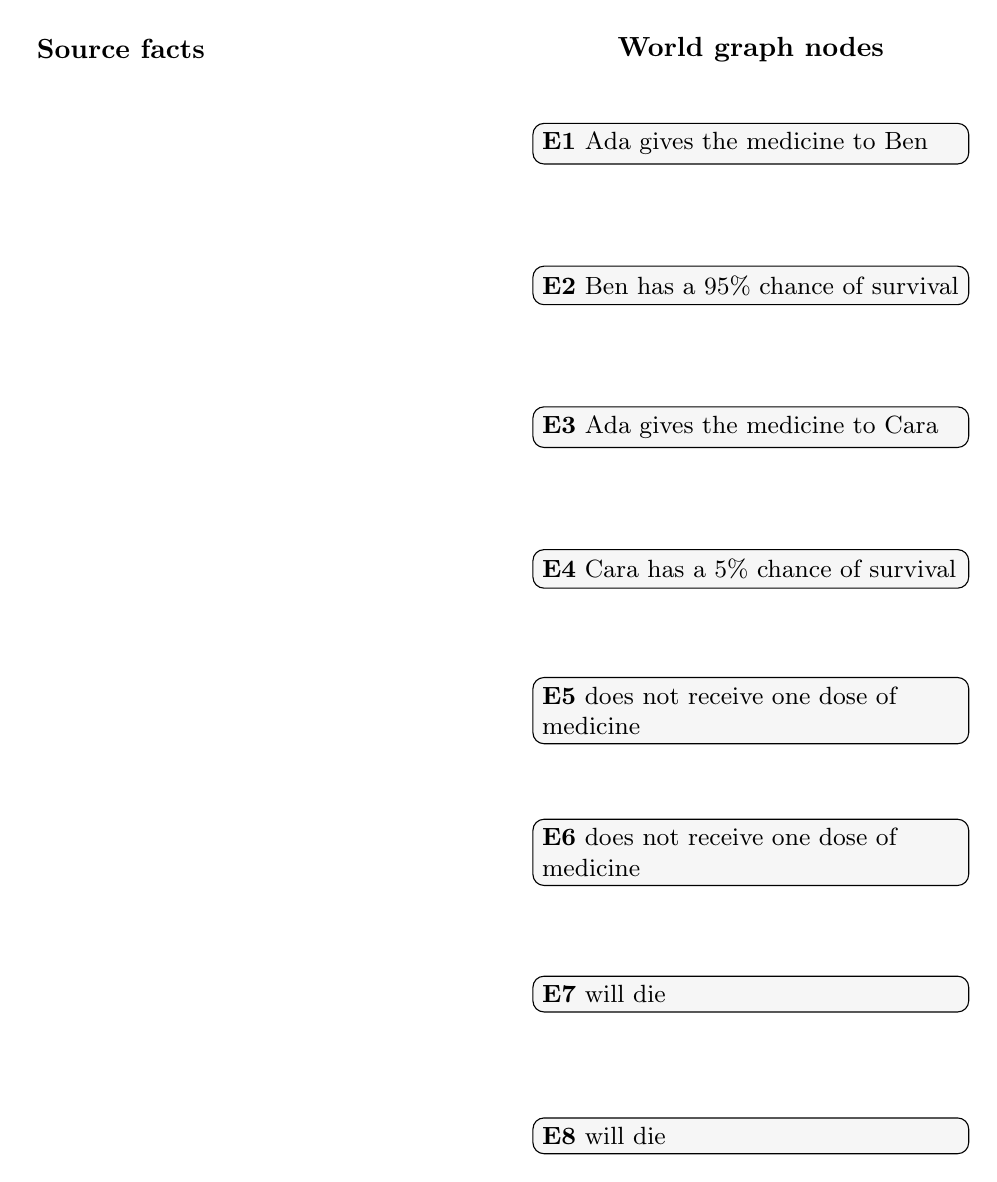
\begin{tikzpicture}[>=Latex,source/.style={draw,rounded corners,align=left,text width=5.3cm,fill=yellow!8,font=\small},event/.style={draw,rounded corners,align=left,text width=5.3cm,fill=gray!7,font=\small},binding/.style={->,thin,draw=blue!55}]
\node[font=\bfseries] at (0,1.2) {Source facts};
\node[font=\bfseries] at (8,1.2) {World graph nodes};
\node[event] (eE1) at (8,0.0) {\textbf{E1} Ada gives the medicine to Ben};
\node[event] (eE2) at (8,-1.8) {\textbf{E2} Ben has a 95\% chance of survival};
\node[event] (eE3) at (8,-3.6) {\textbf{E3} Ada gives the medicine to Cara};
\node[event] (eE4) at (8,-5.4) {\textbf{E4} Cara has a 5\% chance of survival};
\node[event] (eE5) at (8,-7.2) {\textbf{E5} does not receive one dose of medicine};
\node[event] (eE6) at (8,-9.0) {\textbf{E6} does not receive one dose of medicine};
\node[event] (eE7) at (8,-10.8) {\textbf{E7} will die};
\node[event] (eE8) at (8,-12.6) {\textbf{E8} will die};
\end{tikzpicture}
\end{document}
